\documentclass[aspectratio=1610]{beamer}
\usepackage{style}
\graphicspath{{./assets/images}}

\title{Il Corso di Laurea in Informatica}
\author{Filippo Daniotti}
\date{\today}
\logo{
\includegraphics[height=0.8cm]{logo-small.jpg}}
\institute[DISI]{Dipartimento di Ingegneria e Scienza dell'Informazione}

% arara: pdflatex: { shell: yes, synctex: yes }
% arara: latexmk: { clean: partial }
\begin{document}
	\begin{frame}[plain]
		\addtocounter{framenumber}{-1}
		\centering
		
\includegraphics[width=0.5\textwidth, keepaspectratio]{logo-unitn.eps}		
		\titlepage
		% \tableofcontents
	\end{frame}

	\section{Introduzione e contesto}
	\begin{frame}[fragile]{Che cos'è l'informatica?}
		\begin{center}
			\Large{TL;DR}\\
		\end{center}		
		È tante cose, dare una definizione precisa ad alta voce lascia interdetto qualsiasi interlocutore. In un certo senso è quasi più utile parlare di cosa \alert<1>{non} è, questo se non altro ci aiuta a non fare assunzioni sbagliate.\\
		\bigskip
		\pause
		Giusto per puntualizzare quelle che sono di certo ovvietà, l'informatica \emph{non} è:
		\begin{columns}
			\begin{column}{0.55\textwidth}
				\begin{itemize}
					\item l'ECDL 
					\item hackerare i profili social 
					\item preparare le crack per i videogiochi 
					\item riparare i computer \Large{AHHHHHHHH} 
				\end{itemize}		
			\end{column}
			\onslide<3-> {
				\begin{column}{0.4\textwidth}
					% inserire memino qui sul riparare i computer + esprienza 150h
					\begin{figure}
						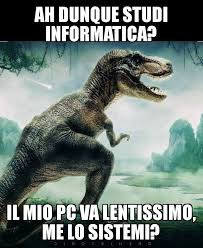
\includegraphics[width=0.5\textwidth, keepaspectratio]{memino.jpg}	
					\end{figure}
				\end{column}
			}
		\end{columns}
	\end{frame}

	\begin{frame}{Daiiii almeno qualcosina per avere un'idea}
		Secondo Wikipedia:
		\begin{quote}
			L'informatica è la scienza che si occupa del trattamento dell'informazione mediante procedure automatizzate[...]
		\end{quote}
		\vfill
		\onslide<2->{
			Lista assolutamente non esaustiva di ambiti e branche dell'informatica
			\begin{itemize}
				\item Algoritmi e strutture dati
				\item Teoria della calcolabilità/complessità/grafi/automi
				\item Reti di calcolatori
				\item Crittografia e sicurezza
				\item Intelligenza artificiale
				\item Ambiti interdisciplinari: bioinformatica, calcolo quantistico, et cetera
			\end{itemize}
		}
	\end{frame}

	\begin{frame}{Super citazione della vita}
		\only<1-3>{
			\begin{center}
				\begin{minipage}{\textwidth}
					\begin{alertblock}{Attenzione}
						Citazione super boomer con immagine a bassa risoluzione e buono kaffè in omaggio in arrivo fra
					\end{alertblock}	
				\end{minipage}
			\end{center}
		}
		\vfill
		\only<1>{\centering\Huge 3...}
		\only<2>{\centering\Huge 2...}
		\only<3>{\centering\Huge 1...}
		\only<4>{
			\begin{figure}
				\centering
				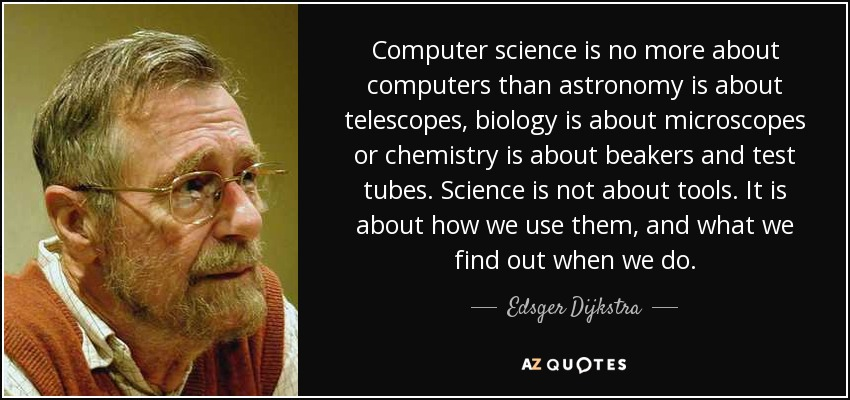
\includegraphics[width=\textwidth, keepaspectratio]{dijkstra.jpg}
			\end{figure}
		}
		\only<5->{
			\begin{figure}
				\centering
				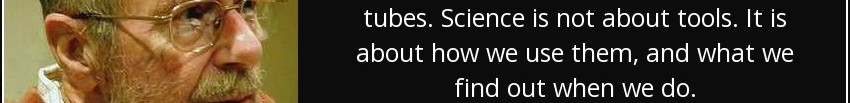
\includegraphics[width=\textwidth, keepaspectratio]{dijkstra-fragment.jpg}
			\end{figure}
			\visible<6>{
			\begin{center}
				\begin{minipage}{\textwidth}
					\begin{block}{Notate quel \emph{Science}}
						Informatica è a tutti gli effetti una laurea \emph{scientifica}
						\begin{center}
							\begin{tabular}{ c c c }
								Laurea in Informatica & \(\to\) & Scienziato \\
								Laurea in Ingegneria Informatica & \(\to\) & Ingegnere
							\end{tabular}
						\end{center}
					\end{block}
				\end{minipage}
			\end{center}
		}
		}
	\end{frame}

\end{document}